\section{Released Evidence for a Provenance Effect}
\label{sec:evidence}
We begin from the public aggregate audit of ReasoningBank on benign AgentDojo Banking endpoints \citep{li2026audit}. The audit separates retrievals according to whether the retrieved memory was derived from a successful episode or from a failed episode. Table~\ref{tab:provenance} reproduces the reported counts after converting the rounded accuracies back to their integer support.

\begin{table}[t]
\centering
\caption{Provenance-conditioned ReasoningBank outcomes from the released financial-agent audit.}
\label{tab:provenance}
\small
\begin{tabular}{lrrr}
\toprule
Retrieved memory provenance & Cases & Correct & Accuracy \\
\midrule
Success-derived & 101 & 94 & 0.931 \\
Failure-derived & 34 & 22 & 0.647 \\
\bottomrule
\end{tabular}
\end{table}

The observed accuracy gap is 28.4 percentage points. This is a large effect at the retrieval stratum level. The transition audit gives the provenance signal a sharper interpretation. ReasoningBank records 25 W$\rightarrow$C recoveries and 9 C$\rightarrow$W regressions. Ten W$\rightarrow$W persistent failures remain after evolution. All ten belong to the failure-derived retrieval stratum.

The rounded provenance accuracies imply 12 failures among 34 failure-derived retrievals and 7 failures among 101 success-derived retrievals. The ten W$\rightarrow$W cases therefore account for roughly 83.3\% of failures in the failure-derived stratum. The success-derived stratum contains no W$\rightarrow$W case in the audit. Figure~\ref{fig:source} visualizes this decomposition.

\begin{figure}[t]
\centering
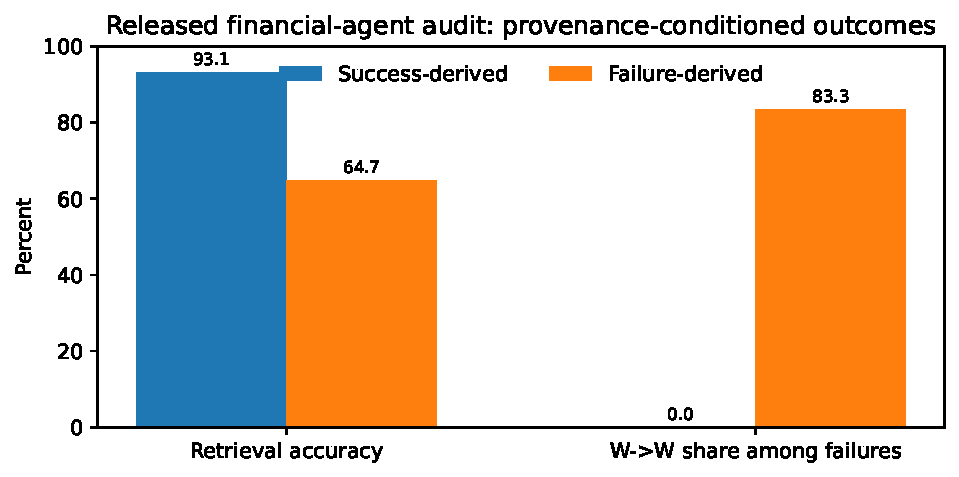
\includegraphics[width=0.95\linewidth]{figures/fig2_source_reanalysis.pdf}
\caption{The released audit shows a large accuracy gap by memory provenance. Persistent W$\rightarrow$W failures are concentrated in failure-derived retrievals.}
\label{fig:source}
\end{figure}

\subsection{The signal is strongest for persistence}
The transition structure changes the scientific interpretation of the aggregate accuracy gap. Failure-derived memory is tightly associated with errors that persist across self-evolution. The source audit identifies task difficulty as a confound for this association. Our causal formulation preserves the persistence signal as the main target and removes task difficulty through an intervention on memory provenance.

A simple arithmetic check sharpens the motivating association. The failure-derived stratum contains roughly two failures beyond the ten W$\rightarrow$W cases, whereas the success-derived stratum contains seven failures. The provenance signal therefore concentrates on persistent error much more strongly than on newly induced regression. We treat this pattern as a reason to audit provenance, not as evidence that failure provenance itself causes persistence.

\subsection{Independent mechanism evidence}
Memory Reward Inflation studies a different memory architecture and identifies an amplification channel for erroneous memories \citep{asadolahi2026inflation}. Incorrect memories can receive inflated utility scores, which increases their future reuse, including under similarity-based retrieval. This illustrates why observed memory reward, retrieval frequency, and source provenance can become entangled. It does not predict a fixed success/failure provenance sign.

Together, the financial-agent audit and reward-inflation results motivate a causal audit of what information provenance contributes beyond memory content. Section~\ref{sec:intervention} first localizes the writer-mode bundle with historical L1 endpoints and then executes the exact-information L2 provenance-exposure contrast.
